\documentclass[main.tex]{subfiles}
\begin{document}

\subsection{$\mathfrak{so}(8)$ Determine which of the representations $(2,2,1,1)\oplus(1,1,2,2)$ and $(2,1,1,2)\oplus(1,2,2,1)$ corresponds to $D^1$ and which corresponds to $D^4$.}
Repeating from the book, $\mathfrak{so}(8)$ has a $\mathfrak{su}(2)\times\mathfrak{su}(2)\times\mathfrak{su}(2)\times\mathfrak{su}(2)$ subalgebra with the four orthogonal roots $\alpha^0=-e^1-e^2,\alpha^1=e^1-e^2,\alpha^3=e^3-e^4,\alpha^4=e^3+e^4$. 

Under the subalgebra on the spinor representation $D^3$ with weights 
\begin{equation}
\eta_je^j/2;\qquad\prod_{j}\eta_j=-1.
\end{equation}
under the subalgebra the 8 weights break into two sets transforming irreducibly under the subalgebra. The set
\begin{equation}\label{eq:set1D3}
\begin{split}
\frac{1}{2}(e^1+e^2+e^3-e^4),&\quad\frac{1}{2}(e^1+e^2-e^3+e^4),\\\frac{1}{2}(-e^1-e^2+e^3-e^4),&\quad\frac{1}{2}(-e^1-e^2-e^3+e^4).
\end{split}
\end{equation}
is orthogonal to $\alpha^1$ and $\alpha^4$ and so transforms like a singlet under the two $\mathfrak{su}(2)$'s associated to $\alpha^1$ and $\alpha^4$ but transforms like a doublet under the $\mathfrak{su}(2)$'s associated to $\alpha^0$ and $\alpha^3$.
Similarly the set
\begin{equation}\label{eq:set2D3}
\begin{split}
\frac{1}{2}(e^1-e^2+e^3+e^4)&,\quad\frac{1}{2}(e^1-e^2-e^3-e^4),\\\frac{1}{2}(-e^1+e^2+e^3+e^4)&,\quad\frac{1}{2}(-e^1+e^2-e^3-e^4)
\end{split}
\end{equation}
is orthogonal to $\alpha^0$ and $\alpha^3$ and transforms trivially under the two $\mathfrak{su}(2)$'s and transforms like a doublet under the $\mathfrak{su}(2)$'s associated with $\alpha^1$ and $\alpha^4$ and so under the subalgebra the representation $D^3$ transforms as $(2,1,2,1)\oplus(1,2,1,2)$

In a similar fashion we can deduce how $D^4$ transforms. The spinor representation $D^4$ has weights
\begin{equation}
\eta_je^j/2;\qquad\prod_{j}\eta_j=1.
\end{equation}
which break up into two sets
\begin{equation}\label{eq:set1D4}
\begin{split}
\frac{1}{2}(e^1+e^2+e^3+e^4)&,\quad\frac{1}{2}(-e^1-e^2-e^3-e^4),\\\frac{1}{2}(+e^1+e^2-e^3-e^4)&,\quad\frac{1}{2}(-e^1-e^2+e^3+e^4)
\end{split}
\end{equation}
is orthogonal to $\alpha^1$ and $\alpha^3$ so the spinor transforms trivially under the $\mathfrak{su}(2)$'s associated to $\alpha^1$ and $\alpha^3$ and transforms like a doublet under the $\mathfrak{su}(2)$'s associated to $\alpha^0$ and $\alpha^4$. 
Likewise, the set 
\begin{equation}\label{eq:set2D4}
\begin{split}
\frac{1}{2}(e^1-e^2+e^3-e^4)&,\quad\frac{1}{2}(-e^1+e^2-e^3+e^4),\\\frac{1}{2}(e^1-e^2-e^3+e^4)&,\quad\frac{1}{2}(-e^1+e^2+e^3-e^4)
\end{split}
\end{equation}
is orthogonal to $\alpha^0$ and $\alpha^4$ so the spinor transforms trivially under the $\mathfrak{su}(2)$'s associated to $\alpha^0$ and $\alpha^4$ and transforms like a doublet under the $\mathfrak{su}(2)$'s associated to $\alpha^1$ and $\alpha^3$. 
Therefore, under the $\mathfrak{su}(2)^0\times\mathfrak{su}(2)^1\times\mathfrak{su}(2)^3\times\mathfrak{su}(2)^4$ subalgebra $D^4$ transforms as
\begin{equation}
(2,1,1,2)\oplus(1,2,2,1).
\end{equation}

The vector representation $D^1$ has weights $\pm e^j$ and so splits into two sets. The weights $\pm e^1$ and $\pm e^2$ form one set orthogonal to $\alpha^3$ and $\alpha^4$. While the other set is composed of $\pm e^3$ and $\pm e^4$ orthogonal to $\alpha^0$ and $\alpha^1$ and therefore, by the same arguments as before, the vector representation $D^1$ transforms as
\begin{equation}
(2,2,1,1)\oplus(1,1,2,2).
\end{equation}

\subsection{Does $SO(8)$ have a $SO(5)$ subgroup under which one spinor $(D^4)$ transforms like two $SO(5)$ spinors while the other spinor $(D^3)$ transforms like an $SO(5)$ vector and three singlets? To DO!}

The Dynkin diagram of $\mathfrak{so}(5)$ or $B_2$ is
\begin{figure}[H] 
\centering
  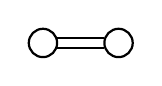
\begin{tikzpicture}[scale=.6]
   \draw[thick] (-1.6,0) circle (.3);
   \draw[thick] (0,0) circle (.3);
   \draw[thick] (-1.3,-0.1  ) -- +(1 ,0);
   \draw[thick] (-1.3,+0.1  ) -- +(1 ,0);
 \end{tikzpicture}
\end{figure}

The two roots have an angle $\theta_{\alpha\beta}=\frac{3\pi}{4}$. Therefore we choose the two $\mathfrak{so}(8)$ roots corresponding to the $\mathfrak{so}(5)$ roots as $\alpha^1=e^1-e^2$ and $\alpha^2=e^2-e^3$ constrained to the $2-d$ space.

%The extended Dynkin diagram $D_4'$ is
%\begin{figure}[H] 
%\centering
%  \begin{tikzpicture}[scale=.6]
 %   \draw (-3.71,1) node[anchor=east]  {$D_4'$};
  %  \draw[thick] (-1.81, 0.21 ) -- +(-0.707 ,0.707);
   % \draw[thick] (-2.73,1.13) circle (.3);
    %\draw[thick] (-1.81, -0.21 ) -- +(-0.707 ,-0.707);
%    \draw[thick] (-2.73,-1.13) circle (.3);
 %   \draw[thick] (-1.6,0) circle (.3);
  %  \draw[thick] (-1.39, 0.21 ) -- +(0.707 ,0.707);
   % \draw[thick] (-0.47,1.13) circle (.3);
  %  \draw[thick] (-1.39, -0.21 ) -- +(0.707 ,-0.707);
  %  \draw[thick] (-0.47,-1.13) circle (.3);
  %\end{tikzpicture}
%\end{figure}
%Removing one of the outside roots (say $\alpha^0$) from the extended Dynkin diagram gives 



\end{document}